 % !TEX encoding = UTF-8 Unicode
% !TeX TXS-program:compile = txs:///pdflatex/[--shell-escape] 

\documentclass[12pt, twoside]{book}
%***************************************************************************************************

% Podstawowe ustawienia języka, według którego formatowany będzie dokument
\usepackage[english]{babel}

% Pakiet babel dla polskiego języka powoduje konflikt z pakietem amssymb.
% Polecenie '\lll' definiują oba pakiety - porządana jest druga definicja.
\let\lll\undefined

% W przypadku wielojęzykowości ustawia główny język dokumentu
\selectlanguage{english}

% Kodowanie dokumentu
% \usepackage[utf8]{inputenc}
% \usepackage[T1]{fontenc}
% \usepackage{lmodern}

% Unicode support for LuaLaTeX
\usepackage{fontspec}
\setmainfont{Latin Modern Roman}
\setsansfont{Latin Modern Sans}
\setmonofont{Latin Modern Mono}

% Polskie wcięcia akapitów
\usepackage{indentfirst}

% Polskie formatowanie typograficzne
\frenchspacing

% Zapewnia liczne usprawnienia wyświetlania i organizacji matematycznych formuł.
\usepackage{amsmath}

% Wprowadza rozszerzony zestaw symboli m.in. \leadsto
\usepackage{amssymb}

% Dodatkowa, ,,kręcona'' czcionka matematyczna
\usepackage{mathrsfs}

% Dodatkowe wsparcie dla środowiska mathbb, które nie wspiera
% domyślnie cyfr (\mathbb{})
%\usepackage{bbold}

% Fixes/improves amsmath
\usepackage{mathtools}

% Markdown
\usepackage[smartEllipses,hybrid]{markdown}

% ***************************************************************************************************
% Kolory
% ***************************************************************************************************

% Umożliwia kolorowanie poszczególnych komórek tabeli
\usepackage[table, svgnames]{xcolor}% http://ctan.org/pkg/

% Umożliwia łatwą zmianę koloru linii w tabeli
\usepackage{tabu}

% Umożliwia rozszerzoną kontrolę nad kolorami.
\usepackage{xcolor}

% Definicje kolorów
\definecolor{lgray}{HTML}{9F9F9F}
\definecolor{dgray}{HTML}{5F5F5F}

% ***************************************************************************************************
% Algorytmy
% ***************************************************************************************************

% Udostępnia środowisko do konstruowania pseudokodów
\usepackage[ruled,vlined,linesnumbered,longend,algochapter]{algorithm2e}

% Zamiana nazwy środowiska z domyślnej "Algorithm X" na "Pseudokod X"
\newenvironment{algorithm-custom}[1][htb]{
  \renewcommand{\algorithmcfname}{Algorithm}
  \begin{algorithm}[#1]%
  }{
  \end{algorithm}
}

% Zmiana rozmiaru komentarzy
\newcommand\algcomment[1]{
  \footnotesize{#1}
}

% Ustawienie zadanego stylu dla komentarzy
\SetCommentSty{algcomment}

% Wyśrodkowana tylda
\usepackage{textcomp}%
\newcommand{\textapprox}{\raisebox{0.5ex}{\texttildelow}}

% Listowanie kodów źródłowych
\usepackage{listings}
\renewcommand{\lstlistingname}{Source code} % Polska nazwa listingu

% ***************************************************************************************************
% Marginesy
% ***************************************************************************************************

% Ustawienia rozmiarów stron i ich marginesów
\usepackage[headheight=18pt, top=25mm, bottom=25mm, left=25mm,
right=25mm]{geometry}

% Usunięcie górnego marginesu dla środowisk
\makeatletter
\setlength\@fptop{0\p@}
\makeatother

% ***************************************************************************************************
% Styl
% ***************************************************************************************************

% Definiuje środowisko 'titlingpage', które zapewnia pełną kontrolę
% nad układem strony tytułowej.
\usepackage{titling}

% Umożliwia modyfikowanie stylu spisu treści
\usepackage[subfigure]{tocloft}

\tocloftpagestyle{tableOfContentStyle}

\setcounter{tocdepth}{1}

% Definiowanie własnych stylów nagłówków i/lub stopek
\usepackage{fancyhdr}

% Domyślny styl dla pracy
\fancypagestyle{custom}{
  \fancyhf{}                  % wyczyść stopki i nagłówki
  \fancyhead[RO]{                % Prawy, nieparzysty nagłówek
    \hrulefill \hspace{16pt} \large Chapter \thechapter
    \put(-471.5,5.5){%
      \makebox(0,0)[l]{%
        \small Wrocław University of Science and Technology
      }
    }
  }
  \fancyhead[LE]{                % Lewy, parzysty nagłówek
    \large Chapter \thechapter \hspace{16pt} \hrulefill
    \put(-267,5.5){%
      \makebox(0,0)[l]{%
        \small Faculty of Information and Communication Technology
      }
    }
  }
  \fancyfoot[LE,RO]{              % Stopki
    \thepage
  }
  \renewcommand{\headrulewidth}{0pt}      % Grubość linii w nagłówku
  \renewcommand{\footrulewidth}{0.2pt}    % Grubość linii w stopce
}

% Domyślny styl dla List of Figures
\fancypagestyle{ListofFiguresStyle}{
  \fancyhf{}                  % wyczyść stopki i nagłówki
  \fancyhead[RO]{                % Prawy, nieparzysty nagłówek
    \hrulefill \hspace{16pt} \large List of Figures
    \put(-471.5,5.5){%
      \makebox(0,0)[l]{%
        \small Wrocław University of Science and Technology
      }
    }
  }
  \fancyhead[LE]{                % Lewy, parzysty nagłówek
    \large List of Figures \hspace{16pt} \hrulefill
    \put(-267,5.5){%
      \makebox(0,0)[l]{%
        \small Faculty of Information and Communication Technology
      }
    }
  }
  \fancyfoot[LE,RO]{              % Stopki
    \thepage
  }
  \renewcommand{\headrulewidth}{0pt}      % Grubość linii w nagłówku
  \renewcommand{\footrulewidth}{0.2pt}    % Grubość linii w stopce
}

% Domyślny styl dla List of Tables
\fancypagestyle{ListofTablesStyle}{
  \fancyhf{}                  % wyczyść stopki i nagłówki
  \fancyhead[RO]{                % Prawy, nieparzysty nagłówek
    \hrulefill \hspace{16pt} \large List of Tables
    \put(-471.5,5.5){%
      \makebox(0,0)[l]{%
        \small Wrocław University of Science and Technology
      }
    }
  }
  \fancyhead[LE]{                % Lewy, parzysty nagłówek
    \large List of Tables \hspace{16pt} \hrulefill
    \put(-267,5.5){%
      \makebox(0,0)[l]{%
        \small Faculty of Information and Communication Technology
      }
    }
  }
  \fancyfoot[LE,RO]{              % Stopki
    \thepage
  }
  \renewcommand{\headrulewidth}{0pt}      % Grubość linii w nagłówku
  \renewcommand{\footrulewidth}{0.2pt}    % Grubość linii w stopce
}

% Domyślny styl dla bibliografii
\fancypagestyle{bibliographyStyle}{
  \fancyhf{}                  % wyczyść stopki i nagłówki
  \fancyhead[RO]{                % Prawy, nieparzysty nagłówek
    \hrulefill \hspace{16pt} \large Bibliography
    \put(-471.5,5.5){%
      \makebox(0,0)[l]{%
        \small Wrocław University of Science and Technology
      }
    }
  }
  \fancyhead[LE]{                % Lewy, parzysty nagłówek
    \large Bibliography \hspace{16pt} \hrulefill
    \put(-267,5.5){%
      \makebox(0,0)[l]{%
        \small Faculty of Information and Communication Technology
      }
    }
  }
  \fancyfoot[LE,RO]{              % Stopki
    \thepage
  }
  \renewcommand{\headrulewidth}{0pt}      % Grubość linii w nagłówku
  \renewcommand{\footrulewidth}{0.2pt}    % Grubość linii w stopce
}

% Domyślny styl dla dodatków
\fancypagestyle{appendixStyle}{
  \fancyhf{}                  % wyczyść stopki i nagłówki
  \fancyhead[RO]{                % Prawy, nieparzysty nagłówek
    \hrulefill \hspace{16pt} \large Appendix \thechapter
    \put(-472.1, 12.1){%
      \makebox(0,0)[l]{%
        \includegraphics[width=0.05\textwidth]{resources/pwr-logo}
      }
    }
    \put(-443,5.5){%
      \makebox(0,0)[l]{%
        \small Wrocław University of Science and Technology
      }
    }
  }
  \fancyhead[LE]{                % Lewy, parzysty nagłówek
    \large Dodatek \thechapter \hspace{16pt} \hrulefill
    \put(-22, 12.1){%
      \makebox(0,0)[l]{%
        \includegraphics[width=0.05\textwidth]{wiz-logo}
      }
    }
    \put(-220,5.5){%
      \makebox(0,0)[l]{%
        \small Faculty of Information and Communication Technology
      }
    }
  }
  \fancyfoot[LE,RO]{              % Stopki
    \thepage
  }
  \renewcommand{\headrulewidth}{0pt}      % Grubość linii w nagłówku
  \renewcommand{\footrulewidth}{0.2pt}    % Grubość linii w stopce
}

% Osobny styl dla stron zaczynających rozdział/spis treści itd.
% (domyślnie formatowane jako "plain")
\fancypagestyle{chapterBeginStyle}{
  \fancyhf{}%
  \fancyfoot[LE,RO]{
    \thepage
  }
  \renewcommand{\headrulewidth}{0pt}
  \renewcommand{\footrulewidth}{0.2pt}
}

% Styl dla pozostałych stron spisu treści
\fancypagestyle{tableOfContentStyle}{
  \fancyhf{}%
  \fancyfoot[LE,RO]{
    \thepage
  }
  \renewcommand{\headrulewidth}{0pt}
  \renewcommand{\footrulewidth}{0.2pt}
}

% Formatowanie tytułów rozdziałów i/lub sekcji
\usepackage{titlesec}

% Formatowanie tytułów rozdziałów
\titleformat{\chapter}[hang]
{\vspace{-10ex}\normalfont\Huge\bfseries}
{\thechapter.}
{1ex}
{}
%[\vspace{2ex}]

% Formatowanie tytułów sekcji
\titleformat{\section}[hang]
{\normalfont\Large\bfseries}
{\thesection.}
{1ex}
{}

\titleformat{\subsection}[hang]
{\normalfont\large\bfseries}
{\thesubsection.}
{1ex}
{}
% formatowanie elementów przed modyfikowanym tytułem

% ***************************************************************************************************
% Linki
% ***************************************************************************************************

% Umożliwia wstawianie hiperłączy do dokumentu
% \usepackage{hyperref}              % MOVED
% \hypersetup{
%   colorlinks  =  true,
%   linkcolor  =  blue,
%   citecolor  =  red,
%   urlcolor  =  blue
% }
% \urlstyle{same}

% ***************************************************************************************************
% Linki
% ***************************************************************************************************

% Umożliwia zdefiniowanie własnego stylu wyliczeniowego
\usepackage{enumitem}

% Nowa lista numerowana z trzema poziomami
\newlist{myitemize}{itemize}{3}

% Definicja wyglądu znacznika pierwszego poziomu
\setlist[myitemize,1]{
  label    =  \textbullet,
leftmargin  =  4mm}

% Definicja wyglądu znacznika drugiego poziomu
\setlist[myitemize,2]{
  label    =  $\diamond$,
leftmargin  =  8mm}

% Definicja wyglądu znacznika trzeciego poziomu
\setlist[myitemize,3]{
  label    =  $\diamond$,
  leftmargin  =  12mm
}

% ***************************************************************************************************
% Inne pakiety
% ***************************************************************************************************

% Dołączanie rysunków
\usepackage{graphicx}

% Figury i przypisy
\usepackage{caption}
\usepackage{subcaption}

% Umożliwia tworzenie przypisów wewnątrz środowisk
\usepackage{footnote}

% Umożliwia tworzenie struktur katalogów
\usepackage{dirtree}

% Rozciąganie komórek tabeli na wiele wierszy
\usepackage{multirow}

% Precyzyjne obliczenia szerokości/wysokości dowolnego fragmentu
% wygenerowanego przez LaTeX
\usepackage{calc}

% ***************************************************************************************************
% Matematyczne skróty
% ***************************************************************************************************

% Skrócony symbol liczb rzeczywistych
\newcommand{\RR}{\mathbb{R}}

% Skrócony symbol liczb naturalnych
\newcommand{\NN}{\mathbb{N}}

% Skrócony symbol liczb wymiernych
\newcommand{\QQ}{\mathbb{Q}}

% Skrócony symbol liczb całkowitych
\newcommand{\ZZ}{\mathbb{Z}}

% Skrócony symbol logicznej implikacji
\newcommand{\IMP}{\rightarrow}

% Skrócony symbol  logicznej równoważności
\newcommand{\IFF}{\leftrightarrow}

% ***************************************************************************************************
% Środowiska
% ***************************************************************************************************

% Środowisko do twierdzeń
\newtheorem{theorem}{Twierdzenie}[chapter]

% Środowisko do lematów
\newtheorem{lemma}{Lemat}[chapter]

% Środowisko do przykładów
\newtheorem{example}{Przykład}[chapter]

% Środowisko do wniosków
\newtheorem{corollary}{Wniosek}[chapter]

% Środowisko do definicji
\newtheorem{definition}{Definicja}[chapter]

% Środowisko do dowodów
\newenvironment{proof}{
  \par\noindent \textbf{Dowód.}
}{
  \begin{flushright}
    \vspace*{-6mm}\mbox{$\blacklozenge$}
  \end{flushright}
}

% Środowisko do uwag
\newenvironment{remark}{
  \bigskip \par\noindent \small \textbf{Uwaga.}
}{
  \begin{small}
    \vspace*{4mm}
  \end{small}
}

% dodatkowe pomagające, oczywiście nie wszystskie są wymagane
\usepackage{psfrag}
\usepackage{amsfonts}
\usepackage{supertabular}
\usepackage{array}
\usepackage{tabularx}
\usepackage{hhline}
% \usepackage{minted}
\usepackage{url}
\usepackage{microtype}
\usepackage{booktabs}
\usepackage{pgfplotstable}
\usepackage{makecell}
\usepackage{rotating}
\usepackage{multicol}
\usepackage{cuted}
\usepackage{colortbl}
\usepackage{adjustbox}
\usepackage{color,soul}
\usepackage{pdfpages}

\let\origdoublepage\cleardoublepage
\newcommand{\clearemptydoublepage}{\clearpage{\pagestyle{empty}\origdoublepage}}
\let\cleardoublepage\clearemptydoublepage

\usepackage{pifont}
\newcommand{\cmark}{\ding{51}}
\newcommand{\xmark}{\ding{55}}
\newcommand{\bftab}{\fontseries{b}\selectfont}

\usepackage[nocompress]{cite}

\newcolumntype{P}[1]{>{\raggedright\arraybackslash\noindent}p{#1}}

\newcolumntype{R}[1]{>{\raggedleft\arraybackslash}p{#1}}
\newcolumntype{L}[1]{>{\raggedright\arraybackslash}p{#1}}
\newcolumntype{C}[1]{>{\centering\arraybackslash}m{#1}}

\usepackage{caption}
\usepackage{url}
\usepackage{color,soul}
\usepackage[inkscapelatex=false]{svg}
\usepackage{tabto}
\usepackage{wrapfig}

% formatowanie pierwszych stron rozdziałów - pomagające
\usepackage{hyperref}              % MOVED HERE
\hypersetup{
  colorlinks  =  true,
  linkcolor  =  blue,
  citecolor  =  red,
  urlcolor  =  blue
}
\urlstyle{same}

\newcommand{\resetformatting}{
  \fancypagestyle{plain}{
    \fancyhf{}%
    \fancyfoot[LE,RO]{
      \thepage
    }
    \renewcommand{\headrulewidth}{0pt}
    \renewcommand{\footrulewidth}{0.2pt}
} }
\newcommand{\doublepage}{
  \newpage
  \thispagestyle{empty}
\cleardoublepage}

\newcommand\Chapter[1]{
  \chapter{#1}
\thispagestyle{chapterBeginStyle}}


\frontmatter
%check the current front page here:
%https://wiz.pwr.edu.pl/en/students/thesis
%and generate pdfs, and save in title_page folder.
\begin{document}


\includepdf[pages={1}]{title_page/pd_mgr_pl.pdf}
\doublepage
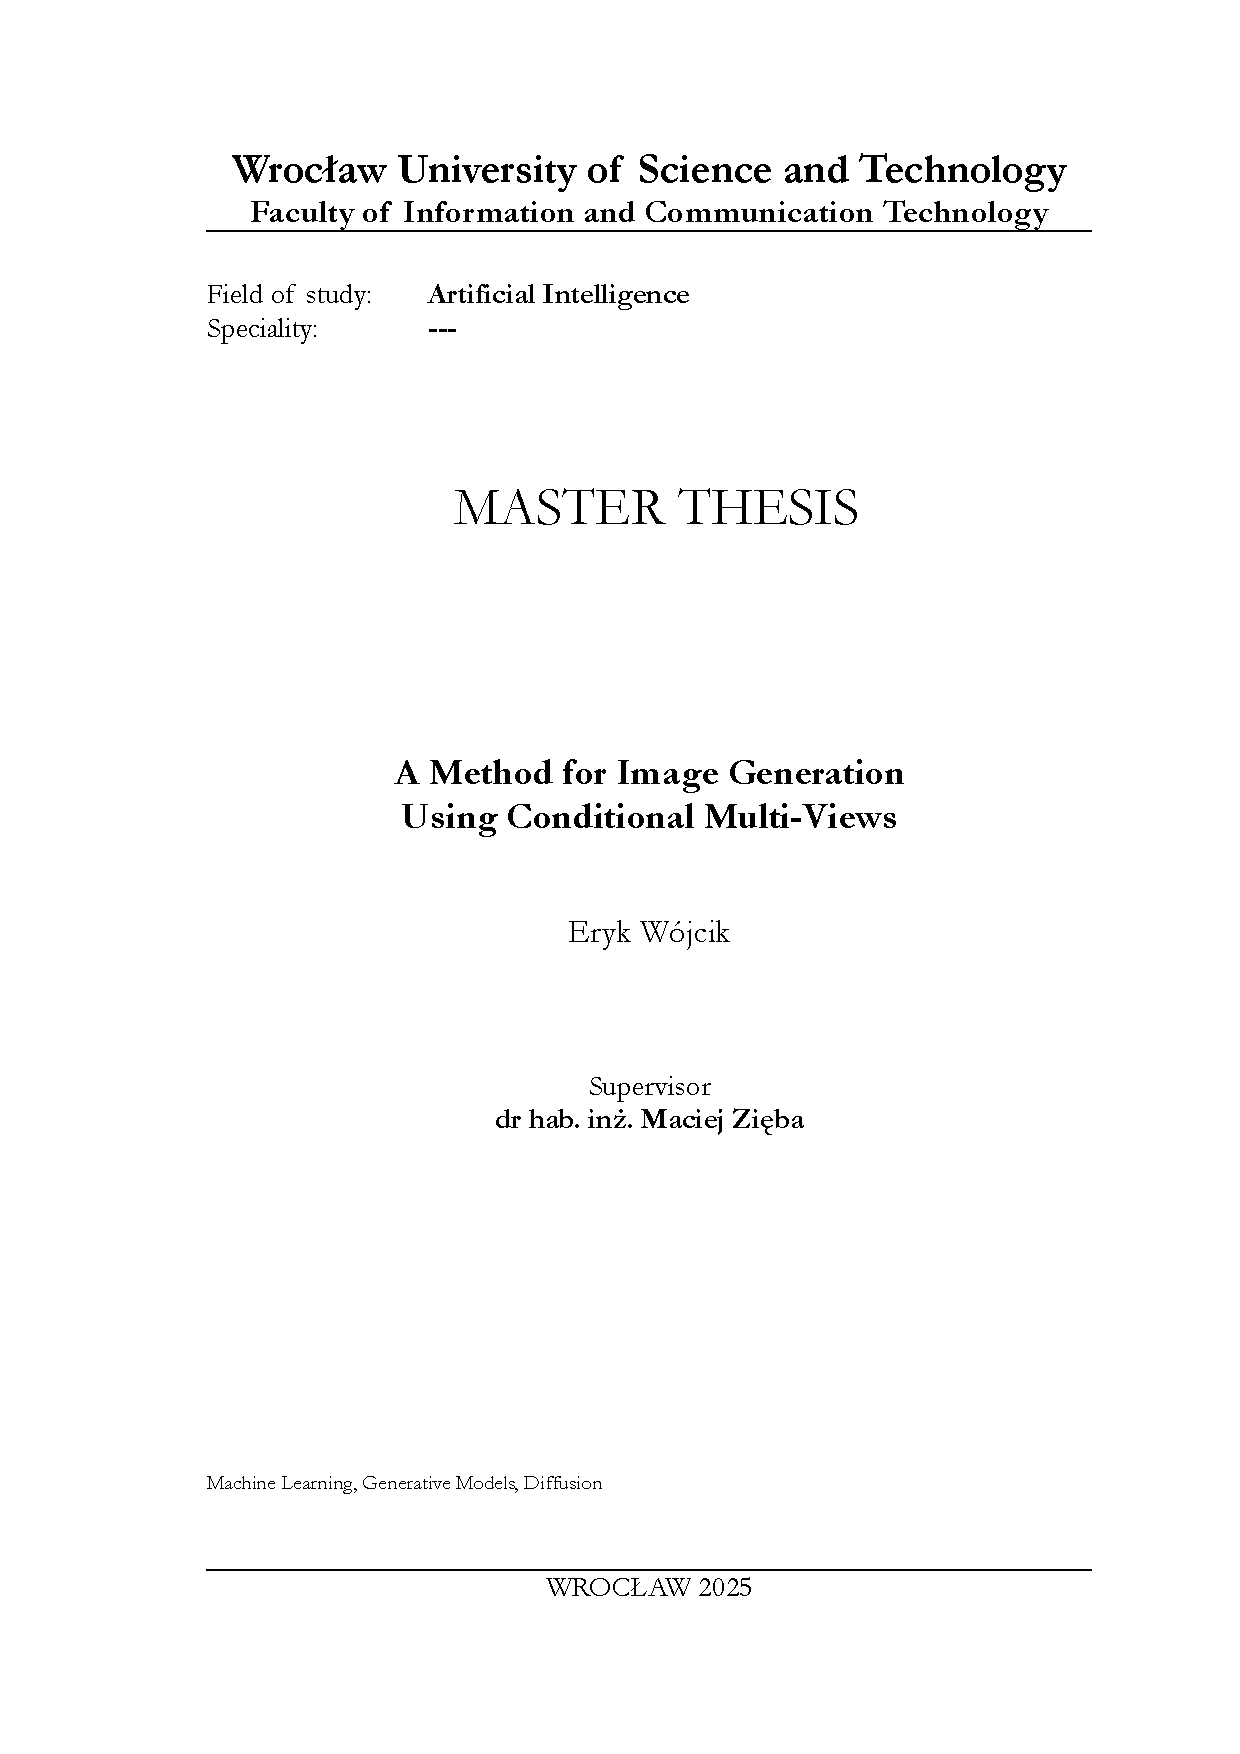
\includepdf[pages={1}]{title_page/pd_mgr_en.pdf}	
\doublepage
% Add table of contents
\pagestyle{tableOfContentStyle}
% Add abstract
\pagenumbering{Roman}
\section*{Streszczenie}

Synteza nowych widoków obiektów na podstawie pojedynczych obrazów pozostaje jednym z najbardziej wymagających problemów w widzeniu komputerowym. Istniejące metody oparte na modelach dyfuzyjnych borykają się z kompromisem między efektywnością obliczeniową a jakością wyników. Niniejsza praca wprowadza nowatorskie podejście łączące Feature-wise Linear Modulation (FiLM) do warunkowania parametrami kamery oraz równoległe adaptery atencji krzyżowej dla warunkowania widokiem referencyjnym.
Proponowana metoda trenuje jedynie $585M$ z $2.9B$ parametrów ($20\%$) przy zachowaniu porównywalnej wydajności z pełnym dostrajaniem modelu, osiągając $4$-krotnie szybsze uczenie. Walidacja na zbiorach danych ObjaverseXL \cite{objaversexl} i Google Scanned Objects \cite{gso} wykazuje korzyści w zakresie efektywności obliczeniowej w porównaniu z najlepszymi metodami Zero123++ \cite{zero1to3} i MVAdapter \cite{mvadapter}, choć z niższą jakością wyników wynikającą z ograniczonej skali danych treningowych.

\section*{Abstract}

Novel view synthesis of objects from single images remains one of the most challenging problems in computer vision. Existing diffusion-based methods face a trade-off between computational efficiency and result quality. This work introduces a novel approach combining Feature-wise Linear Modulation (FiLM) for camera parameter conditioning with parallel cross-attention adapters for visual conditioning.
The proposed method trains only $585M$ of $2.9B$ parameters ($20\%$) while achieving comparable performance to full model fine-tuning, with $4\times$ faster training. Validation on ObjaverseXL \cite{objaversexl} and Google Scanned Objects \cite{gso} datasets demonstrates computational efficiency benefits compared to state-of-the-art Zero123++ \cite{zero1to3} and MVAdapter \cite{mvadapter} methods, though with performance gaps attributable to constrained training data scale.

\doublepage
\tableofcontents 
\doublepage
% Set page style 
\pagestyle{custom}
\mainmatter
 
% Create chapters:
\Chapter{Introduction}\label{chapter:introduction}

\section{Motivation}

Novel view synthesis from single images remains one of computer vision's most challenging problems. While diffusion models have revolutionized 2D image generation, adapting them for 3D-aware synthesis poses fundamental challenges: how to effectively encode geometric transformations without disrupting pre-trained knowledge, and how to balance computational efficiency with model expressiveness.

Current approaches suffer from critical limitations. Methods like Zero-1-to-3 \cite{zero1to3} use simple pose vectors that provide insufficient geometric detail for complex viewpoint changes. Advanced techniques like CAT3D \cite{cat3d} and MV-Adapter \cite{mvadapter} rely on complex raymap representations that are likely to introduce visual artifacts and struggle with reflective materials. Meanwhile, most of the existing methods require full fine-tuning large diffusion models which is computationally prohibitive.

This work addresses a fundamental question: \textit{Can we achieve effective 3D conditioning in diffusion models while maintaining computational efficiency and visual quality?}

\section{Contributions}

In this work, I introduce a novel approach that combines Feature-wise Linear Modulation (FiLM) for camera parameter conditioning with parallel image cross-attention adapters for visual conditioning. My key contributions are:

\begin{enumerate}
  \item \textbf{FiLM-based camera conditioning}: First application of FiLM to camera parameter encoding in diffusion models, providing direct geometric control without visual artifacts.
  \item \textbf{Hybrid conditioning architecture}: A dual-stream approach combining global geometric modulation with selective visual attention, addressing fundamental trade-offs in novel view synthesis.
  \item \textbf{Efficient adapter training}: Training only $585M$ of $2.9B$ parameters (20\%) while achieving comparable performance to full fine-tuning, with $4\times$ faster training.
  \item \textbf{Systematic evaluation}: Comprehensive ablation studies and comparison with state-of-the-art methods, demonstrating effectiveness across metrics and datasets.
\end{enumerate}

Proposed method achieves competitive results with Zero123++ \cite{zero1to3} and MVAdapter \cite{mvadapter} while requiring significantly fewer computational resources and producing fewer visual artifacts.

\section{Research Questions}

This work addresses four specific research questions:
\begin{itemize}
  \item Can Feature-wise Linear Modulation (FiLM) provide an effective alternative to complex raymap representations for camera parameter encoding?
  \item Can a hybrid conditioning strategy combining visual and geometric information achieve superior results compared to existing single-modal approaches?
  \item What is the optimal balance between training efficiency and model expressiveness in adapter-based approaches for novel view synthesis?
  \item How can we effectively condition the diffusion process to generate novel views of objects from a single reference image?
\end{itemize}

\section{Structure}

Chapter 2 reviews related work in 3D reconstruction, diffusion models, and novel view synthesis. Chapter 3 details the proposed method, including theoretical justification and architectural design. Chapter 4 describes data preparation with emphasis on lighting consistency between rendered images. Chapter 5 presents experimental evaluation including ablation studies and comparisons with state-of-the-art methods. Chapter 6 concludes with limitations, and future work.

\Chapter{Related Work}\label{chapter:related}

In this chapter, I provide a comprehensive review of existing
approaches relevant to multi-view image generation.

The chapter begins by introducing the fundamental task of Novel View
Synthesis (NVS) and its significance. We then delve into traditional
3D reconstruction techniques (Section \ref{sec:3d-reconstruction})
and their inherent limitations, particularly for sparse-input
scenarios, which motivates the exploration of generative methods.
Subsequently, the discussion shifts to the foundational principles of
Deep Generative Models for Image Synthesis, with a focus on diffusion
models (Section \ref{sec:text-to-image}).

Building on this, we explore various methods for Conditioning
Diffusion Models for Enhanced Control and New Tasks (Section
\ref{sec:conditioning-diffusion}), including the crucial role of
camera parameter encoding and the concept of lightweight adaptation
through adapters.

The core of the chapter then examines state-of-the-art
Diffusion-based Multi-View Image Generation techniques (Section
\ref{sec:multi-view-diffusion}), covering both single reference image
novel view synthesis and architectures for coherent multi-view
generation, including specialized multi-view adapters.
%  Finally, the chapter will conclude with a summary of the discussed
% methods and highlight identified research gaps that this thesis
% aims to address.

\section{Traditional 3D Reconstruction Approaches}\label{sec:3d-reconstruction}

Simultaneous Localization and Mapping (SLAM) is a fundamental concept
in the field of computer vision and robotics. It refers to the
process of simultaneously estimating the camera's position and
orientation in a 3D environment while mapping the environment itself.
Originally, SLAM was used to track the position of a robot in a 3D
space, but it has since been applied to a wide range of problems,
including augmented reality, medical applications and novel view
synthesis.

SLAM works by processing sensor data in real-time to create a map of the unknown environment while simultaneously tracking the position of the sensor within that map. This process typically involves several key steps:
\begin{enumerate}
  \item \textbf{Feature Detection}: Identifying distinctive points or features in the environment from sensor data
  \item \textbf{Data Association}: Matching observed features with previously mapped features
  \item \textbf{State Estimation}: Updating the estimated pose of the camera and the map of the environment
  \item \textbf{Loop Closure}: Recognizing when the sensor has returned to a previously visited location and adjusting the map accordingly to reduce accumulated errors
\end{enumerate}

To address these requirements, researchers have
concentrated on creating techniques for machines to independently
build ever more precise scene representations. This integration of
robotics, computer vision, sensor technology, and recent advancements
in artificial intelligence has shaped this field.

Typically, SLAM techniques use a combination of data sources, such as
images, laser range scans, sonars and GPS to effectively map an environment.
In this work I will focus on the use of images for 3D reconstruction.

\subsection{Structure from Motion Pipeline}

One of the most popular methods for 3D reconstruction from images is
COLMAP \cite{colmap}. COLMAP is a general-purpose
structure-from-motion (SfM) \cite{multipleviewgeometry} system that
can automatically reconstruct 3D scenes from a collection of images.
It is a popular choice for 3D reconstruction due to its accuracy,
speed, and ease of use.

\begin{figure}[h]
  \centering
  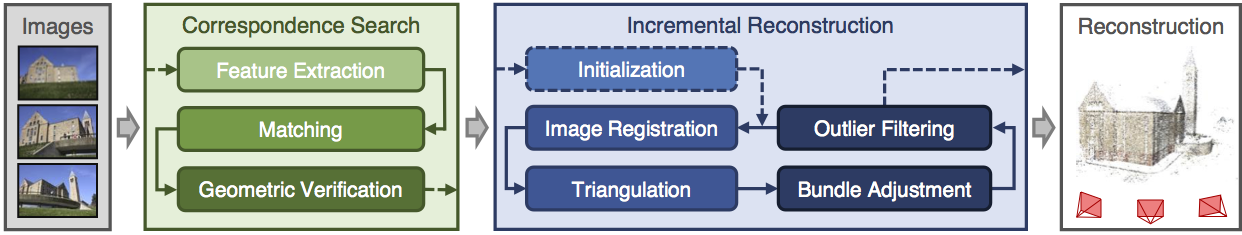
\includegraphics[width=0.9\textwidth]{images/related-work/COLMAP.png}
  \caption{COLMAP pipeline}
  \label{fig:colmap-pipeline}
  % https://colmap.github.io/tutorial.html
\end{figure}

Structure from Motion works in two main steps [Figure
\ref{fig:colmap-pipeline}]:
\begin{enumerate}
  \item \textbf{Correspondence Search}: Identify the unique landmarks
    (features) in all of the images and match the same landmarks across images.
  \item \textbf{Incremental Reconstruction}: Estimates the camera
    poses and triangulates 3D points through an iterative process.
\end{enumerate}

First step of correspondence search is feature extraction. COLMAP
uses SIFT \cite{sift} and ORB \cite{orb} methods to extract features
from images. Scale-invariant feature transform (SIFT) is a method for
detecting keypoints that contrast with their surroundings and
describing the local image content around them. It is invariant to
rotation and scale, making it robust for matching features across images taken from different viewpoints and distances. Oriented FAST and Rotated BRIEF (ORB) is a more
computationally efficient alternative to SIFT, combining a high-speed
FAST detector with optimized descriptors for rotation invariance,
offering comparable matching performance with significantly reduced computational requirements.

\begin{figure}[h]
  \centering
  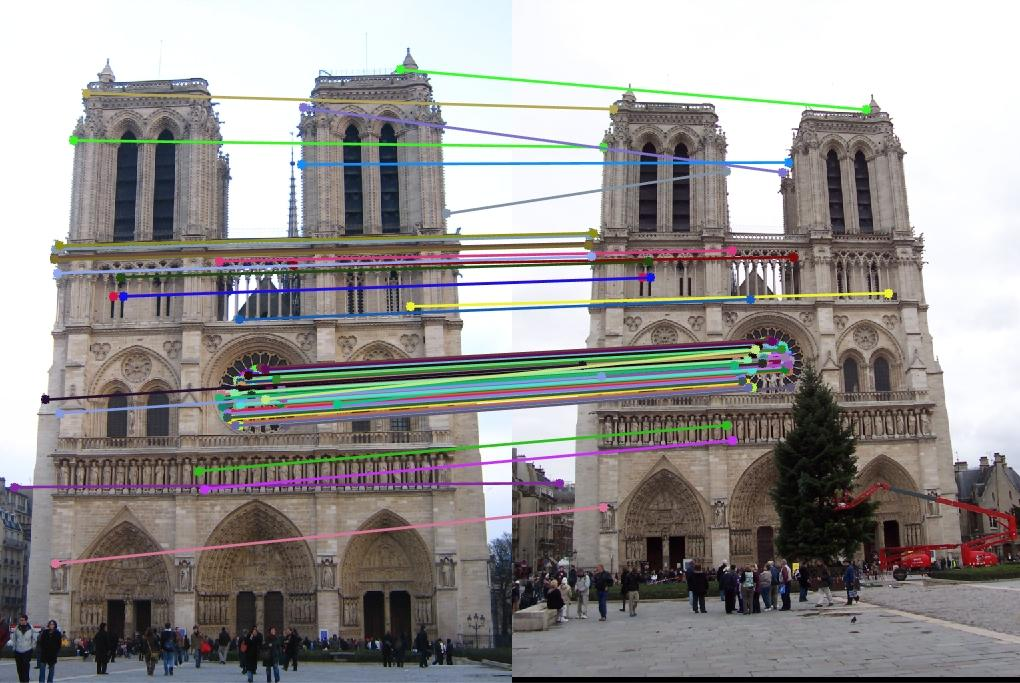
\includegraphics[width=0.7\textwidth]{images/related-work/feature-matching.jpg}
  \caption{Feature matching result}
  \label{fig:matching-features}
  % https://blog.roboflow.com/image-matching/
\end{figure}

Second step is matching features across images. Feature matching is a
process of finding the best matches of features across the images.
COLMAP uses a variant of the FLANN \cite{flann} library to find the
best matches for each feature. FLANN is a library for performing fast
approximate nearest neighbor searches in high dimensional spaces.
Feature matching is visualized in Figure \ref{fig:matching-features}.

Then the geometric verification step uses the prior knowledge about
the camera model and motion to remove outliers, preparing the
verified feature matches for the subsequent Incremental Reconstruction phase.

When it comes to Incremental Reconstruction, the process is as follows:
\begin{enumerate}
  \item \textbf{Camera Pose Estimation}: Estimate the camera location
    and direction in 3D space for each image.
  \item \textbf{Triangulation}: Triangulate 3D points of the observed
    objects from the camera poses and matched features.
  \item \textbf{Bundle Adjustment}: Refine the camera poses and 3D
    points to minimize the reprojection error.
\end{enumerate}

\begin{figure}[h]
  \centering
  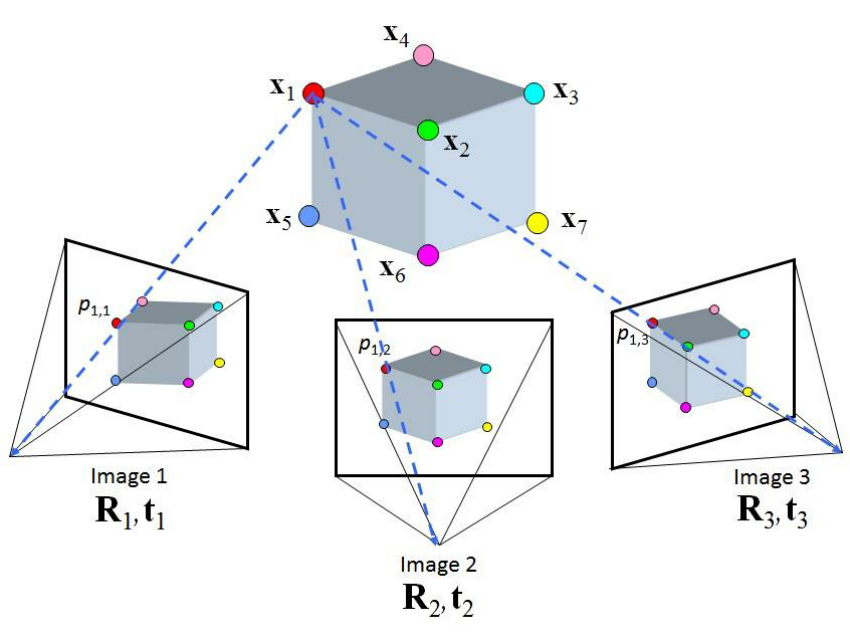
\includegraphics[width=0.5\textwidth]{images/related-work/Structure-from-Motion-SfM-process-is-illustrated-The-structure-in-the.png}
  \caption{Camera pose estimation}
  \label{fig:camera-pose-estimation}
  % https://www.researchgate.net/figure/Structure-from-Motion-SfM-process-is-illustrated-The-structure-in-the_fig2_269327935
\end{figure}

The camera pose estimation (visualized in Figure
\ref{fig:camera-pose-estimation}) starts with an initialization step,
where the initial pair of images and matched features between them
are used to estimate the camera pose. Then, the algorithm proceeds to
the loop (Figure \ref{fig:colmap-pipeline}), where the next image is
registered to the reconstruction and the camera pose is estimated
again (triangulation step). After that the bundle adjustment step is
performed to refine the camera poses and 3D points to be consistent
with the entire dataset with images of a given scene. This
optimization process typically uses the Levenberg-Marquardt algorithm
to minimize reprojection error. This process is repeated for each
subsequent batch of images, updating the camera poses and 3D points.

\subsection{Methods for 3D Reconstruction}

The field of 3D reconstruction encompasses various approaches beyond the basic Structure from Motion pipeline. These methods can be broadly categorized into two groups: sparse reconstruction (like SfM) and dense reconstruction methods.

\subsubsection{Dense Reconstruction Methods}

While SfM provides camera poses and a sparse point cloud, dense reconstruction methods aim to create a complete 3D model with detailed surface information. Notable methods include:

\begin{enumerate}
  \item \textbf{Multi-View Stereo (MVS)}: After obtaining camera poses through SfM, MVS algorithms like PMVS \cite{pmvs} generate dense point clouds by matching pixels across multiple images.

  \item \textbf{Depth Map Fusion}: Methods such as COLMAP's MVS pipeline estimate per-image depth maps and then fuse them into a consistent 3D model.

  \item \textbf{Neural Radiance Fields (NeRF)} \cite{nerf}: A more recent approach that represents scenes as continuous 5D functions (spatial location and viewing direction) encoded in neural networks. NeRF takes camera poses from SfM as input and uses ray tracing to synthesize novel views with remarkable detail and view consistency.
\end{enumerate}

\subsubsection{Learning-based Reconstruction}

Recent approaches leverage deep learning for 3D reconstruction, often using SfM-derived data for supervision or initialization:

\begin{enumerate}
  \item \textbf{Learned MVS}: Methods like MVSNet \cite{mvsnet} use convolutional neural networks to learn the depth estimation process directly from images and camera parameters.

  \item \textbf{Single-view Reconstruction}: Networks like Mesh R-CNN \cite{meshrcnn} can estimate 3D structure from a single image by leveraging prior knowledge learned from large datasets.
\end{enumerate}

\subsection{Limitations of 3D Reconstruction}

Structure from Motion is a powerful tool for 3D reconstruction, demonstrating high effectiveness across a variety of scenarios. However, it encounters significant challenges. These include dealing with textureless surfaces, reflective materials, and the computational complexity of processing high-resolution images. Most importantly in the context of this thesis, it struggles with sparse input scenarios, such as those involving a single image or only a few images.

Traditional 3D reconstruction methods like SfM and MVS typically require a dense collection of images with sufficient overlap to establish accurate feature correspondences and camera pose estimations. When faced with limited input views—particularly in the extreme case of a single image—these methods often fail to generate complete and accurate 3D representations. The quality of reconstruction degrades significantly due to:

\begin{enumerate}
  \item \textbf{Geometric ambiguity}: A single image or sparse set of images provides incomplete information about occluded regions and depth, leading to ambiguous geometry.

  \item \textbf{Feature matching limitations}: Fewer images means fewer opportunities to establish reliable feature correspondences across different viewpoints.

  \item \textbf{Inability to triangulate}: Robust triangulation requires features to be visible from multiple viewpoints, which is not possible with very limited inputs.

  \item \textbf{View-dependent effects}: Materials with specular reflections or varying appearance based on viewpoint cannot be accurately modeled without multiple observations.
\end{enumerate}

These limitations have motivated the development of generative approaches to novel view synthesis, particularly using diffusion models trained on large datasets of rendered images of 3D models. Instead of explicitly reconstructing geometry, these methods leverage the power of deep learning to hallucinate plausible views from unseen perspectives.

\begin{figure}[h]
  \centering
  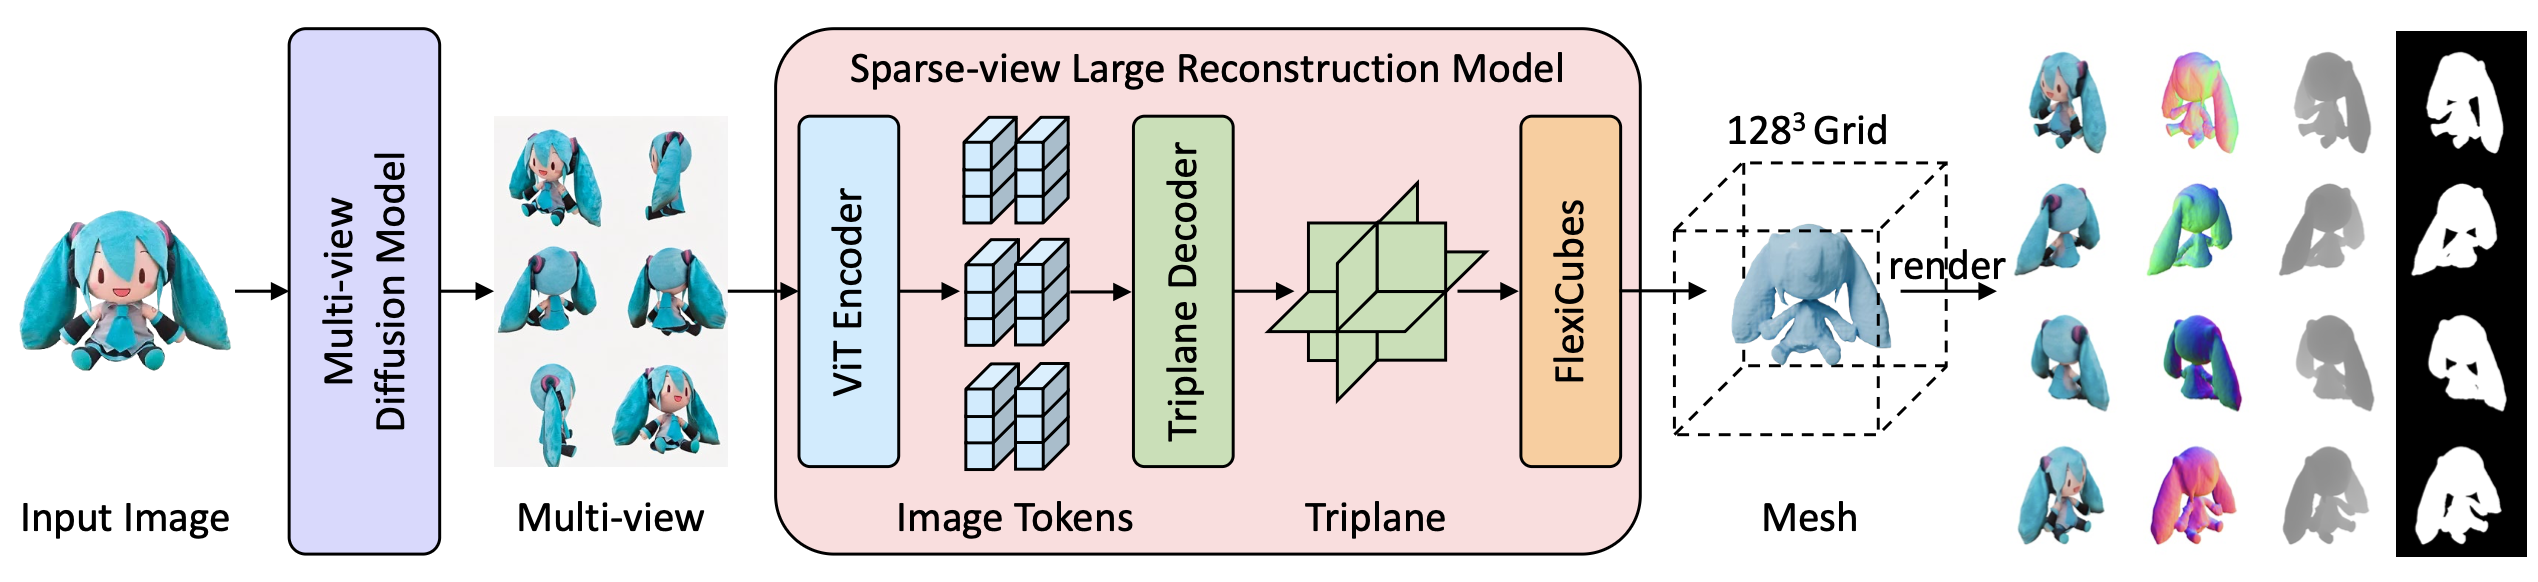
\includegraphics[width=\textwidth]{images/related-work/instantmesh.png}
  \caption{InstantMesh}
  \label{fig:instantmesh}
\end{figure}

Modern approaches of 3D object generation, such as InstantMesh \cite{instantmesh}, leverage these diffusion models to generate multiple consistent views of an object from minimal input (a single image or even a text prompt). This novel view synthesis is the first step in a pipeline \ref{fig:instantmesh} that can be used to create a 3D model of the object, and it is this particular step that forms the central focus of this thesis.

\section{Deep Generative Models for Image Synthesis}\label{sec:text-to-image}

The development of deep learning methods has led to remarkable progress in generative modeling, enabling the synthesis of highly realistic and diverse images. Among the various approaches, Generative Adversarial Networks (GANs), Variational Autoencoders (VAEs), and Diffusion Models have emerged as the most prominent. While GANs and VAEs have laid significant groundwork and continue to be influential, this section will primarily focus on diffusion models, given their state-of-the-art performance in image quality and controllability, and their direct relevance to the multi-view synthesis tasks explored in this thesis.

\subsection{Generative Adversarial Networks (GANs) and Variational Autoencoders (VAEs)}

Generative Adversarial Networks (GANs) \cite{gan} consist of two neural networks, a generator and a discriminator, trained in a competitive setting. The generator aims to produce realistic images, while the discriminator tries to distinguish between real images from the training dataset and fake images produced by the generator. Through this adversarial process, the generator learns to create increasingly plausible images. GANs are known for generating sharp images but often suffer from training instability.

Variational Autoencoders (VAEs) \cite{vae} are another class of generative models that learn a probabilistic mapping from a high-dimensional data space (e.g., images) to a lower-dimensional latent space, and then back to the data space. A VAE consists of an encoder that compresses the input data into a latent representation (typically a mean and variance defining a Gaussian distribution) and a decoder that reconstructs the data from samples drawn from this latent distribution. They are trained to maximize the evidence lower bound (ELBO), which involves a reconstruction loss and a regularization term (KL divergence) that encourages the latent space to be smooth and well-behaved. VAEs generally offer more stable training than GANs and can learn a meaningful latent space, but often produce slightly blurrier images. VAEs play a crucial role in the architecture of Latent Diffusion Models.

\subsection{Diffusion Models}
Diffusion models have recently become the dominant paradigm in high-fidelity image generation. They are inspired by non-equilibrium thermodynamics, specifically diffusion processes.

\subsubsection{Core Concept: The Diffusion Process}
The core idea behind diffusion models involves two processes: a forward (or diffusion) process and a reverse (or denoising) process.
In the \textbf{forward process}, a known image $x_0$ from the dataset is gradually perturbed by adding small amounts of Gaussian noise over a sequence of $T$ steps. This process progressively corrupts the image until, at step $T$, it becomes indistinguishable from pure isotropic Gaussian noise. The parameters of this noising process are fixed.

The \textbf{reverse process} aims to learn to reverse this noising. Starting from pure noise (equivalent to $x_T$), a neural network is trained to gradually denoise the signal, step-by-step, eventually producing a realistic image (an approximation of $x_0$). This learned denoising process is what allows the model to generate new images. Figure \ref{fig:diffusion-process} illustrates this concept.

\begin{figure}[h]
  \centering
  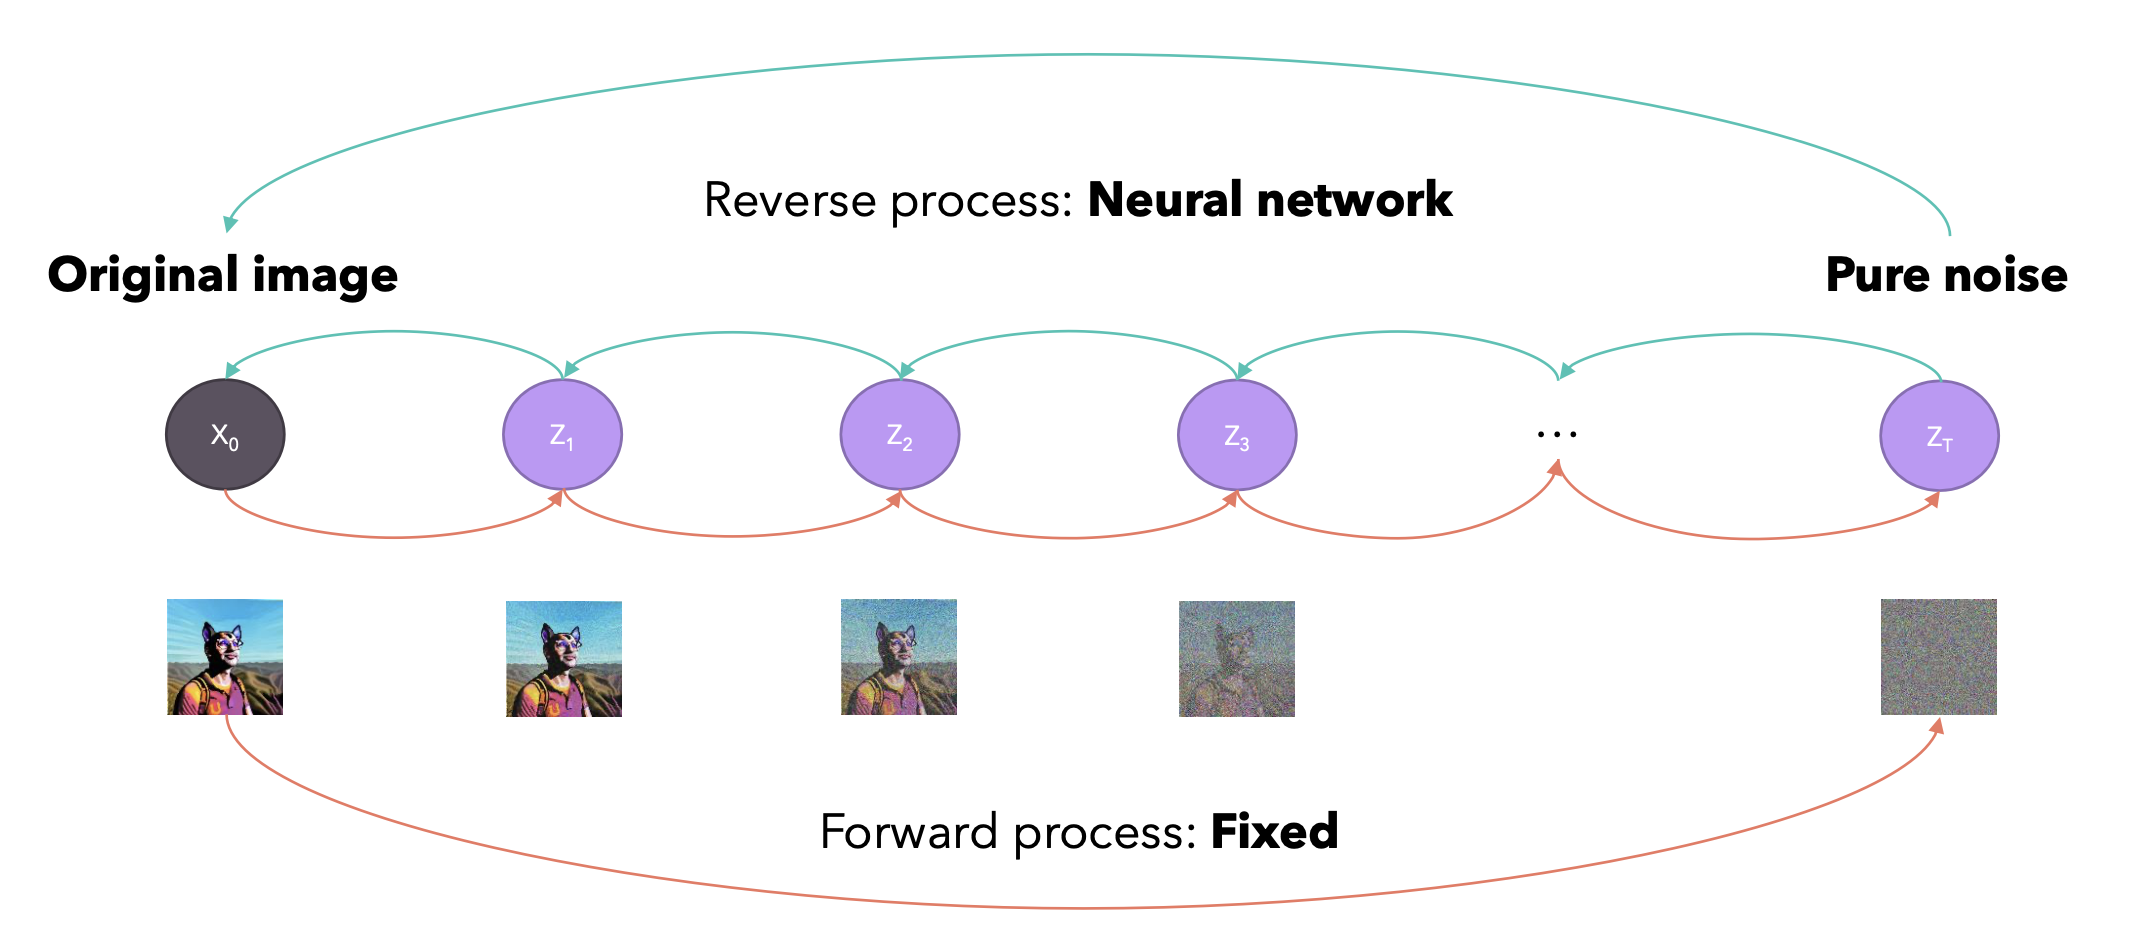
\includegraphics[width=0.8\textwidth]{images/related-work/diffusion-process.png}
  \caption{The forward (noising) and reverse (denoising/generation) stages of a diffusion model. The forward process gradually adds noise to an image until it becomes pure noise. The reverse process learned by a neural net to denoise, step-by-step, to generate an image from noise.}
  \label{fig:diffusion-process}
\end{figure}

\subsubsection{The U-Net Architecture}
The neural network responsible for predicting the noise (or the denoised image) at each step in the reverse process is typically a U-Net architecture \cite{unet}. The U-Net, originally developed for biomedical image segmentation, features an encoder-decoder structure with skip (residual) connections. The encoder path progressively downsamples the input, capturing contextual information, while the decoder path progressively upsamples, localizing information. The skip connections concatenate features from the encoder to corresponding layers in the decoder, allowing the network to combine high-level semantic information with low-level detail, which is crucial for accurately predicting the noise and preserving image fidelity during the denoising steps.

\subsubsection{Training Objective and Loss Function}
The training objective of the diffusion model is to learn the conditional probability distribution $p_\theta(x_{t-1}|x_t)$, which represents the probability of the previous, less noisy state $x_{t-1}$ given the current noisy state $x_t$. In practice, this is often simplified to training the U-Net to predict the noise $\epsilon$ that was added to an image $x_0$ to produce $x_t$ at a given timestep $t$. The loss function is typically the Mean Squared Error (MSE) between the true added noise $\epsilon$ and the noise $\epsilon_\theta(x_t, t)$ predicted by the U-Net:
\[ L = \mathbb{E}_{t \sim [1, T], x_0 \sim q(x_0), \epsilon \sim \mathcal{N}(0, I)} [\|\epsilon - \epsilon_\theta(x_t, t)\|^2] \]
where $x_t = \sqrt{\bar{\alpha}_t}x_0 + \sqrt{1-\bar{\alpha}_t}\epsilon$, and $\bar{\alpha}_t$ are parameters from the noise schedule.

\subsubsection{Conditional Generation: Text-to-Image Synthesis}
To guide the image generation process, diffusion models can be conditioned on various inputs, most notably text prompts. This is the foundation of text-to-image synthesis.
A crucial component for text conditioning is a powerful text encoder that can convert textual descriptions into rich numerical representations (embeddings). Contrastive Language-Image Pre-training (CLIP) \cite{clip} is widely used for this purpose. CLIP is trained on a massive dataset of image-text pairs to learn a shared embedding space where semantically similar images and texts are close together.

The text embeddings from CLIP are then integrated into the U-Net, typically using cross-attention mechanisms. In these layers, the image representation at an intermediate layer of the U-Net queries the text embedding, allowing the model to align parts of the image with relevant words or phrases in the prompt. This enables fine-grained control over the generated image content based on the textual input.

\subsection{Latent Diffusion Models (LDMs)}\label{ssec:ldm}
While standard diffusion models operate directly in the pixel space of images, this can be computationally very expensive, especially for high-resolution images, as the U-Net needs to process large tensors. Latent Diffusion Models (LDMs) \cite{stablediffusion}, such as Stable Diffusion, address this challenge by performing the diffusion and denoising process in a lower-dimensional latent space.

LDMs employ a pre-trained autoencoder, typically a VAE. The VAE's encoder first compresses a high-resolution image from pixel space into a compact latent representation. The diffusion process (both forward and reverse) then occurs entirely within this latent space. Once the reverse denoising process generates a target latent representation from noise, the VAE's decoder maps this latent representation back into the high-resolution pixel space to produce the final image. Figure \ref{fig:ldm-architecture} depicts the architecture of an LDM.

\begin{figure}[h]
  \centering
  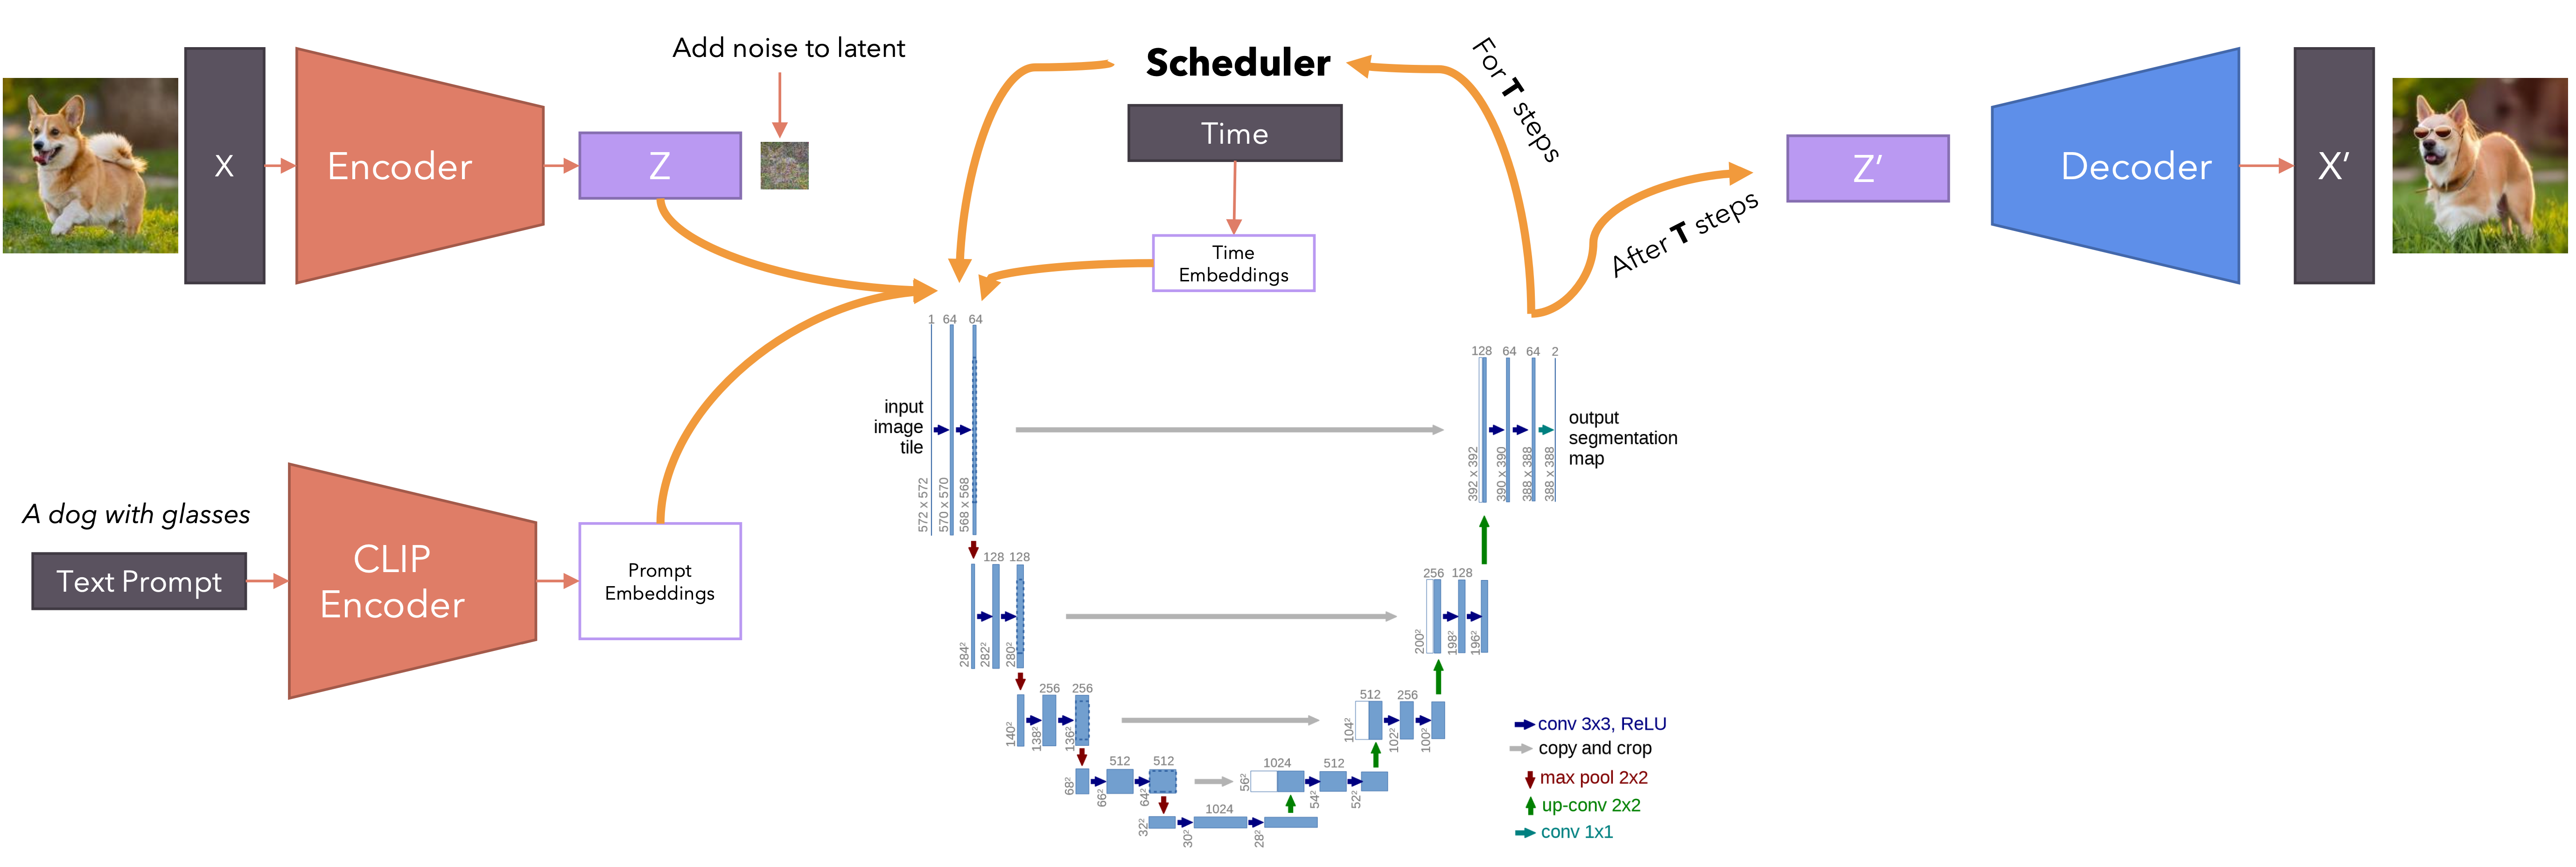
\includegraphics[width=\textwidth]{images/related-work/LDM-detailed.png}
  \caption{Architecture of a Latent Diffusion Model (LDM). An image is first encoded into a latent space by a VAE encoder. The diffusion process (noising and denoising via U-Net) occurs in this latent space. The generated latent is then decoded back to pixel space by the VAE decoder. Conditioning, such as text embeddings from CLIP, is incorporated into the U-Net.}
  \label{fig:ldm-architecture}
\end{figure}

By working in a compressed latent space, LDMs significantly reduce the computational burden during training and inference compared to pixel-space diffusion models. This makes it feasible to train powerful models on massive datasets and generate high-resolution images more efficiently, without a substantial loss in quality. The VAE ensures that the latent space is perceptually equivalent to the pixel space, and the diffusion model learns to generate high-quality latents within this space.

\section{Conditioning Diffusion Models for Enhanced Control and New
Tasks}\label{sec:conditioning-diffusion}

\subsection{Diverse Conditioning Signals}

\subsection{Camera Parameter Encoding for 3D Awareness}

\subsection{Lightweight Adaptation}

To address the limitations of full fine-tuning approaches, recent
works have explored adapter-based methods that allow for more
efficient adaptation of pre-trained models to specific tasks while
preserving their original capabilities.

Adapters are lightweight modules that can be inserted into
pre-trained models to adapt them to new tasks without modifying the
original network parameters. This approach has gained popularity in
natural language processing and has also been applied to diffusion
models for various image generation tasks.

ControlNet \cite{controlnet} introduced a method to add spatial
conditioning to text-to-image diffusion models by training additional
control modules that are connected to the original UNet backbone.
This approach allows for precise control over the generated images
while preserving the original model's capabilities.

Similarly, T2I-Adapter \cite{t2iadapter} proposed a more modular
approach where adapters are trained separately and can be combined to
provide multiple forms of control simultaneously. These methods have
demonstrated the effectiveness of adapter-based approaches for
controlled image generation.

\section{Diffusion-based Multi-View Image
Generation}\label{sec:multi-view-diffusion}

\subsection{Single Reference Image Novel View Synthesis}

Zero-1-to-3 \cite{zero1to3} pioneered the approach of conditioning
diffusion models on both a reference image and camera pose
information to generate novel views. This method demonstrated the
potential of leveraging pre-trained text-to-image models for novel
view synthesis without requiring explicit 3D reconstruction. However,
it often struggles with maintaining geometric consistency across
generated views.

\subsection{Coherent Multi-View Generation Architectures}
% Camera encoding

To address the limitations of single-view approaches, several works
have focused on developing multi-view diffusion models that can
generate multiple consistent views simultaneously.

MVDream \cite{mvdream} extends the self-attention mechanism in
diffusion models to operate across multiple views, enabling the
generation of 3D-consistent images. By jointly modeling multiple
views, this approach significantly improves geometric consistency
compared to methods that generate each view independently.

Similarly, ViewCrafter \cite{viewcrafter} combines video latent
diffusion models \cite{videolatentdiffusion} with 3D point cloud
priors to generate high-fidelity and consistent novel views. By
leveraging the explicit 3D information provided by point clouds and
the generative capabilities of video diffusion models, ViewCrafter
achieves precise control of camera poses and generates high-quality novel views.

CAT3D \cite{cat3d} takes a different approach by simulating a
real-world capture process with a multi-view diffusion model. Given
one or three input images and a set of target novel viewpoints, this
model generates highly consistent novel views that can be used as
input to robust 3D reconstruction techniques.

While these multi-view diffusion models have shown impressive
results, they typically require full fine-tuning of pre-trained
text-to-image models, which is computationally expensive and may lead
to degradation in image quality due to the scarcity of high-quality 3D data.

\subsection{Specialized Multi-View Adapters}

Building upon the success of adapter mechanisms, MV-Adapter
\cite{mvadapter} introduced the first adapter-based solution for
multi-view image generation. Unlike previous approaches that make
invasive modifications to pre-trained text-to-image models and
require full fine-tuning, MV-Adapter enhances these models with a
plug-and-play adapter that preserves the original network structure
and feature space.

MV-Adapter employs a decoupled attention mechanism, where the
original spatial self-attention layers are retained, and new
multi-view attention layers are created by duplicating the structure
and weights of the original layers. These layers are organized in a
parallel architecture, allowing the adapter to inherit the powerful
priors of the pre-trained self-attention layers while efficiently
learning geometric knowledge.

Additionally, MV-Adapter introduces a unified condition encoder that
seamlessly integrates camera parameters and geometric information,
facilitating applications such as text and image-based 3D generation
and texturing. By updating fewer parameters, MV-Adapter enables
efficient training and preserves the prior knowledge embedded in
pre-trained models, mitigating overfitting risks.

problems of the current MVD:
- inconsistant lighting
- poor geometric consistency
- big model training requirements
\Chapter{Chapter 1 TODO}\label{chapter:chapter1}

Politechnika Wrocławska to państwowa uczelnia techniczna we Wrocławiu. Figure~\ref{fig:logo} przedstawia logo uczelni. 
 
\begin{figure}[h]
\centering

\includegraphics[width=0.9\textwidth]{images/LogoPWr.png}
\caption{Logo Politechniki Wrocławskiej}\label{fig:logo}
\end{figure}

Pamiętaj by nie zostawiać pustych miejsc pod tytułem rozdziału. Należy pamiętać o wprowadzeniu. Dopiero później powinny zostać przedstawione podrozdziały.

\section{Tytuł podrozdziału}\label{chapter:podrozdzial}
Praca może zawierać także tabele, które powinny być czytelne i dobrze opisane. Do wszystkich tabel i rysunków powinny pojawić się odwołania w tekście (oraz komentarze). Podpisy rysunków mają znaleźć się pod rysunkami, a podpisy tabel – nad tabelami. Tabela~\ref{tab:tab_example} stanowi przykład. 

\begin{table}[H]
    \centering
        \caption{Krótki ale treściwy opis tabeli} \label{tab:tab_example} 
        \begin{tabular}{lrrrr}
        \toprule
        Method &  anger &   joy &  optimism &  sadness \\
        \midrule
        model1 & 0.772 & \textbf{0.751} & \textbf{0.532} & 0.673 \\
        model2 & 0.727 & 0.661 & 0.307 & 0.629 \\
        model3 & 0.761 & 0.739 & 0.498 & \textbf{0.679} \\
        model4 & \textbf{0.782} & 0.740 & 0.470 & 0.672 \\
        \bottomrule
        \end{tabular}
\end{table}

Warto także użyć gotowych generatorów do tabel (np. \url{https://www.tablesgenerator.com/}), niż formatować je samodzielnie. Mistrzem formatowania był Wojtek. Tabela~\ref{tab:main_results_sentence} o nieco zmienionej treści pochodzi z jego pracy. 

\begin{table}[H]
\centering
\renewcommand*{\arraystretch}{1.3}
\caption{Comparison of the compression methods considered for MultiEmo for the sentence level in the mixed domain scenario. The results are averaged on 5 repetitions. The best results are in \textbf{bold}.}
\label{tab:main_results_sentence}
\begin{tabular}{@{}
l
R{1.3cm}R{0.7cm}@{\hspace{0.1cm}}L{1.1cm}@{\hspace{8pt}}
R{1.3cm}c@{\hspace{12pt}}
cccc
@{}} 
\toprule
\multicolumn{1}{c}{\textbf{Method}} &
\multicolumn{1}{c}{\textbf{$\boldsymbol{\#}$Par.}} & 
\multicolumn{2}{c@{\hspace{12pt}}}{
\begin{tabular}[c]{@{}c@{}}\textbf{Mem.}\\\textbf{ [MB]}\end{tabular}} &
\begin{tabular}[c]{@{}c@{}}\textbf{Train.}\\\textbf{ [min]}\end{tabular} & 
\textbf{Eval [s]} & 
\textbf{Acc.} &
\textbf{F1}& 
\textbf{Rec.}&
\textbf{Prec.} \\ 
\midrule
Model$_\mathrm{BASE}$ & 109M & \multicolumn{2}{c@{\hspace{10pt}}}{418} & 26.0 & 13.9 & 78.8 & 74.7 & 74.1 & 75.8 \\ 
\midrule
Model1 & 67M & 255 & (1.6x) & 14.1 & 7.0 (2.0x) & 77.9 & 73.9 & 73.3 & \bftab{74.8} \\
Model2 & \bftab{13M} & \bftab{49} & \bftab{(8.6x)} & 6.5 & 2.3 (6.2x) & 76.7 & 72.4 & 71.7 & 73.9 \\
Model3$_{6, \mathrm{TA}}$ & 67M & 255 & (1.6x) & 14.1 & 7.2 (1.9x) & 77.7 & 73.8 & 73.5 & 74.3 \\
Model3$_{6, \mathrm{TS}}$ & 68M & 258 & (1.6x) & 62.9 & 7.2 (1.9x) & \bftab{78.2} & \bftab{74.4} & \bftab{74.1} & 74.7 \\
Model3$_{4, \mathrm{TA}}$ & 14M & 55 & (7.6x) & \bftab{5.5} & 2.1 (6.6x) & 76.3 & 72.0 & 71.1 & 73.7 \\
Model3$_{4, \mathrm{TS}}$ & 15M & 56 & (7.5x) & 38.3 & \bftab{2.0 (6.9x)} & 76.3 & 72.2 & 71.5 & 73.4 \\
Model4 & 67M & 255 & (1.6x) & 19.1 & 7.8 (1.8x) & 76.6 & 72.5 & 72.1 & 73.2 \\
Model5 & 14M & 55 & (7.6x) & 121.5 & 3.4 (4.1x) & 77.5 & 72.9 & 72.2 & 74.9 \\
\bottomrule
\end{tabular}
\end{table}

\subsection{Tytuł podpodrozdziału}
Studia zapewniają podstawową wiedzę z zakresu sztucznej inteligencji i nauki o danych (data science). Rozwijają zarówno umiejętności matematyczne, programistyczne, obliczeniowe, analityczne, jak i umiejętności pracy projektowej w grupie, z nastawieniem na identyfikowanie problemów (naukowych, biznesowych, społecznych) i ich rozwiązywanie z wykorzystaniem technik i metod inteligentnych.

\section{Tytuł podrozdziału 2}
Społeczeństwo w swoim rozwoju wchodzi w czwartą rewolucję przemysłową, określaną często terminem ,,Przemysł 4.0''. Jest on oparty na systemach łączności piątej i wyższych generacji oraz Internecie Rzeczy (IoT), wspieranych sztuczną inteligencją.

Przemysł 4.0 zmienia nie tylko technologie, ale przede wszystkim model biznesu i wymagania stawiane pracownikom. Rewolucja oprze się na danych, które będą zbierane, gromadzone i przetwarzane na każdym etapie prowadzenia biznesu. W firmach wykorzystywane będą nowoczesne technologie, chmury obliczeniowe, wielkie zbiory danych, Internet Rzeczy, rozszerzona rzeczywistość, sztuczna inteligencja czy druk 3D.

Technologia powinna uwzględniać właściwe współdziałanie z człowiekiem. Dlatego należy badać aspekty komunikacji i interakcji człowiek – komputer czy szerzej: człowiek i rozbudowane środowiska robotyczne. Bariery rozwoju Przemysłu 4.0 mają związek przede wszystkim z dostępem do wykształconych kadr. To zrozumiałe w obliczu dużych oczekiwań co do interdyscyplinarnych kompetencji stawianych inżynierom.

Nauka przed wyzwaniami
Przyszłość stawia przed europejską nauką trzy kluczowe wyzwania:

\begin{itemize}
    \item Rozwój innowacji zakłócających – innowacje przełomowe, takie które zmienią istniejący porządek na rynku, wprowadzając coś zupełnie nowego.
    \item Biologizacja techniki – zastosowanie praw biologicznych, rządzących procesami zachodzącymi w organizmach żywych, do innych dziedzin.
    \item Bezpieczeństwo publiczne – nowe rozwiązania jakościowe i innowacje dotyczące: bezpieczeństwa w zakresie IT (m.in. w kontekście ataków cybernetycznych), bezpieczeństwa systemów transportu drogowego, kolejowego i lotniczego, bezpieczeństwa infrastrukturalnego miast i zaopatrzenia w wodę i elektryczność.
\end{itemize}

Badania i dydaktyka na wysokim poziomie
Szczególna rola w przełamywaniu barier rozwoju Przemysłu 4.0 przypadnie uniwersytetom, które w swoich zadaniach statutowych mają: badania naukowe i kształcenie na wysokim poziomie.
Zadania te są równie ważne. Nie ma bowiem wysokiej jakości nauczania bez prowadzenia badań naukowych. Nie ma badań naukowych i rozwoju gospodarki bez odpowiednio wykształconej kadry. To uczelnie będą przełamywały główne bariery czwartej rewolucji przemysłowej. Wśród tych uczelni – biorąc pod uwagę kapitał ludzki i społeczny, infrastrukturę badawczą i dydaktyczną – nie może zabraknąć Politechniki Wrocławskiej, aspirującej do bycia uczelnią badawczą. Te istotne zadania w pokonywaniu barier realizują wydziały. Na nie, a przede wszystkim na nowo powstały Wydział Informatyki i Telekomunikacji, spada odpowiedzialność w tej dziedzinie.

Wydział tworzą katedry pochodzące z wydziałów Politechniki Wrocławskiej: Elektroniki, Informatyki i Zarządzania oraz Podstawowych Problemów Techniki.
Badania naukowe prowadzone będą w katedrach: Automatyki, Mechatroniki i Systemów Sterowania, Informatyki Technicznej, Systemów i Sieci Komputerowych, Telekomunikacji i Teleinformatyki, Informatyki i Inżynierii Systemów, Informatyki Stosowanej, Inteligencji Obliczeniowej, Podstaw Informatyki.

Oznacza to, że swoim zakresem obejmą większość dziedzin bezpośrednio związanych z Przemysłem 4.0. Realizowane będą zarówno badania podstawowe, jak i wdrożeniowe, skupimy się także na aktywnej współpracy z gospodarką i komercjalizacji wyników. W/w katedry są gwarancją, że badania obejmą większość dziedzin bezpośrednio związanych z Przemysłem 4.0.

Za cel stawiamy sobie przede wszystkim zapewnienie przyjaznych warunków do rozwoju naukowego, zwłaszcza młodym, oraz przejrzystą ścieżkę kariery naukowej. Badania będziemy prowadzić we wszystkich dyscyplinach powiązanych z informatyką.

Kadra ma świadomość, że fundamentem wydziału jest – stojące na wysokim poziomie, nowoczesne, spełniające potrzeby zmieniającego się świata – nauczanie. Odbywać się ono będzie na 12 polsko- i anglojęzycznych kierunkach: Computer Science, Computer Security, Cyberbezpieczeństwo, Informatyczne Systemy Automatyki, Informatyka Algorytmiczna, Informatyka Stosowana, Informatyka Techniczna, Inżynieria Systemów, Sztuczna Inteligencja, Teleinformatyka, Telekomunikacja, Zaufane Systemy Sztucznej Inteligencji. Lista kierunków będzie sukcesywnie modyfikowana w odpowiedzi na wyzwania stawiane przez uwarunkowania społeczno-gospodarcze.

\Chapter{Conclusions}\label{chapter:conclusions}

This thesis presents a novel approach to diffusion-based novel view synthesis combining FiLM-based camera conditioning with adapter-based training. This chapter summarizes the key findings, discusses limitations, and outlines future research directions.

\section{Summary of Findings}

\begin{enumerate}
  \item \textbf{Hybrid conditioning strategy} combining visual and geometric information shows internal consistency improvements, with optimal configuration ($img\_ref\_scale=1.0$, $cam\_mod\_strength=1.0$) demonstrating complementary information fusion, though overall performance significantly lags behind established methods like Zero123++.

  \item \textbf{Adapter-based training} achieves computational efficiency gains, training only $585M$ parameters ($20\%$ of full model) with $4\times$ faster training time, but this efficiency comes at the cost of synthesis quality, as evidenced by substantial performance gaps in quantitative evaluation.

  \item \textbf{FiLM-based camera conditioning} provides a computationally efficient alternative to complex raymap representations, though the achieved FID scores of 45-50 remain substantially higher than state-of-the-art methods, indicating limited synthesis quality despite artifact reduction compared to raymap approaches.

  \item \textbf{Dual-stream conditioning mechanism} demonstrates architectural feasibility for processing reference images through parallel conditioning streams, though the resulting novel views show significant quality limitations when compared to contemporary approaches.
\end{enumerate}

\section{Limitations and Areas for Improvement}

The experimental results reveal fundamental performance limitations that must be acknowledged:

\textbf{Resolution Constraints}: The current implementation operates at a maximum resolution of $768 \times 768$ pixels, which may be insufficient for applications requiring high-detail novel view synthesis.

\textbf{Single-Object Focus}: The method is primarily designed and evaluated for single-object novel view synthesis. Extension to complex scenes would require architectural modifications and different training strategies.

\textbf{Limited Viewpoint Range}: While the training data covers comprehensive viewpoint distributions 6, 8 or 12 views, extreme viewpoint changes (such as complete 180-degree rotations or significant elevation changes) may still pose challenges for geometric consistency, particularly for objects with complex occlusions or view-dependent materials.

\textbf{Constrained Training Scale and Generalization}: The most significant limitation is the substantial disparity in training data compared to state-of-the-art methods. While the proposed method used 20,000 Objaverse samples, Zero123++ was trained on 800K+ Objaverse models with approximately 10M rendered images - representing a 40$\times$ difference in 3D  model diversity and 100$\times$ difference in training scale. This fundamental data limitation constrains the model's ability to generalize across diverse object types not well-represented in the limited training set, explaining much of the observed performance gap.

\textbf{Inference Speed}: While competitive with similar methods, the 16-second inference time may be prohibitive for real-time applications or interactive systems requiring immediate novel view generation.

\section{Future Research Directions}

Several promising directions emerge from recent research:

\begin{itemize}
  \item \textbf{Advanced architectural foundations}: Adapting the proposed FiLM-based conditioning to modern diffusion transformer architectures (Stable Diffusion 3 \cite{stable_diffusion_3, diffusion_transformers}) could potentially improve synthesis quality through more powerful attention mechanisms, text enrichment, flow matching and scaling properties.

  \item \textbf{Integrated 3D reconstruction pipelines}: Developing hybrid systems that combine explicit 3D reconstruction with generative synthesis could leverage both geometric and generative methods, reconstructing coarse 3D representations then using diffusion models to generate high-quality details such as Human3Diffusion \cite{human3diffusion}.

  \item \textbf{Multi-view consistency and real-time optimization}: Future work could explore stronger geometric constraints for coherent multi-view synthesis and investigate model distillation or quantization for real-time applications in VR/AR and interactive systems.
\end{itemize}

The work presented in this thesis explores the potential of efficient adapter-based approaches for diffusion-based novel view synthesis, though the results highlight significant challenges in achieving competitive performance. While the demonstrated FiLM-based camera conditioning and hybrid adapter architectures offer computational efficiency benefits, the substantial quality gaps compared to established methods—largely attributable to the 40$\times$ smaller training dataset—indicate that efficiency gains are insufficient to compensate for limited training data scale in practical novel view synthesis applications. The systematic experimental framework and performance evaluation provide valuable insights for the research community, particularly in understanding the limitations of adapter-based approaches and the continued need for more sophisticated architectures or training strategies to achieve state-of-the-art synthesis quality.

% Redefine plain for 1st bibliography page style
\resetformatting
% Please read :
%https://www.overleaf.com/learn/latex/Bibliography_management_with_bibtex
\pagestyle{bibliographyStyle}
\bibliographystyle{abbrv}
\bibliography{bibliography}

% Add list of figures and tables
\pagestyle{custom}
\newpage
\pagestyle{ListofFiguresStyle}
\listoffigures
\newpage
\pagestyle{ListofTablesStyle}
\listoftables
\end{document}